\documentclass{amsart}

\newcommand{\cA}{\mathcal{A}}\newcommand{\cB}{\mathcal{B}}
\newcommand{\cC}{\mathcal{C}}\newcommand{\cD}{\mathcal{D}}
\newcommand{\cE}{\mathcal{E}}\newcommand{\cF}{\mathcal{F}}
\newcommand{\cG}{\mathcal{G}}\newcommand{\cH}{\mathcal{H}}
\newcommand{\cI}{\mathcal{I}}\newcommand{\cJ}{\mathcal{J}}
\newcommand{\cK}{\mathcal{K}}\newcommand{\cL}{\mathcal{L}}
\newcommand{\cM}{\mathcal{M}}\newcommand{\cN}{\mathcal{N}}
\newcommand{\cO}{\mathcal{O}}\newcommand{\cP}{\mathcal{P}}
\newcommand{\cQ}{\mathcal{Q}}\newcommand{\cR}{\mathcal{R}}
\newcommand{\cS}{\mathcal{S}}\newcommand{\cT}{\mathcal{T}}
\newcommand{\cU}{\mathcal{U}}\newcommand{\cV}{\mathcal{V}}
\newcommand{\cW}{\mathcal{W}}\newcommand{\cX}{\mathcal{X}}
\newcommand{\cY}{\mathcal{Y}}\newcommand{\cZ}{\mathcal{Z}}
\newcommand{\C}{\mathbb{C}}


\newcommand{\bA}{\mathbb{A}}\newcommand{\bB}{\mathbb{B}}
\newcommand{\bC}{\mathbb{C}}\newcommand{\bD}{\mathbb{D}}
\newcommand{\bE}{\mathbb{E}}\newcommand{\bF}{\mathbb{F}}
\newcommand{\bG}{\mathbb{G}}\newcommand{\bH}{\mathbb{H}}
\newcommand{\bI}{\mathbb{I}}\newcommand{\bJ}{\mathbb{J}}
\newcommand{\bK}{\mathbb{K}}\newcommand{\bL}{\mathbb{L}}
\newcommand{\bM}{\mathbb{M}}\newcommand{\bN}{\mathbb{N}}
\newcommand{\bO}{\mathbb{O}}\newcommand{\bP}{\mathbb{P}}
\newcommand{\bQ}{\mathbb{Q}}\newcommand{\bR}{\mathbb{R}}
\newcommand{\bS}{\mathbb{S}}\newcommand{\bT}{\mathbb{T}}
\newcommand{\bU}{\mathbb{U}}\newcommand{\bV}{\mathbb{V}}
\newcommand{\bW}{\mathbb{W}}\newcommand{\bX}{\mathbb{X}}
\newcommand{\bY}{\mathbb{Y}}\newcommand{\bZ}{\mathbb{Z}}

\newcommand{\pt}{\partial}
\newcommand{\ol}{\overline}

\usepackage{lmodern}
\usepackage[dvipsnames,svgnames,x11names,hyperref]{xcolor}
\usepackage{url,verbatim,amssymb,enumerate,stmaryrd,bbm,mathtools,microtype}
\usepackage[pagebackref,colorlinks,citecolor=Mahogany,linkcolor=Mahogany,urlcolor=Mahogany,filecolor=Mahogany]{hyperref}
\usepackage{setspace}
\setstretch{1.08}

\usepackage{tikz,tikz-cd}
\usetikzlibrary{matrix,calc,positioning,arrows,decorations.pathreplacing,patterns,knots}

\newtheorem{theorem}{Theorem}[section]
\newtheorem{lemma}[theorem]{Lemma}
\newtheorem{proposition}[theorem]{Proposition}
\newtheorem{corollary}[theorem]{Corollary}
\newtheorem*{corollary*}{Corollary}
\newtheorem{conjecture}[theorem]{Conjecture}
\newtheorem{metatheorem}[theorem]{Meta-theorem}
\newtheorem{theoreminprogress}[theorem]{Theorem-in-progress}
\theoremstyle{definition}
\newtheorem{notation}[theorem]{Notation}
\newtheorem{convention}[theorem]{Convention}
\newtheorem{definition}[theorem]{Definition}
\newtheorem{problem}{Problem}
\theoremstyle{remark}
\newtheorem{example}[theorem]{Example}
\newtheorem{remark}[theorem]{Remark}
\newtheorem{warning}[theorem]{Warning}
\newtheorem{question}[theorem]{Question}
\newtheorem{discussion}[theorem]{Discussion}
\renewcommand*{\proofname}{Solution}
\usepackage{wrapfig,caption}
\captionsetup{
	font=small}
\newcommand{\cat}[1]{\mathsf{#1}}
\newcommand{\mr}[1]{{\rm #1}}

\renewcommand\labelitemi{{\boldmath$\cdot$}}

\title[CS124 Programming 2]{Programming PSET 2 - CS 124}
\author{Kevin Patel}
\date{\today}


\begin{document}
\maketitle
\section{Determining the Crossover point}
\flushleft
This first felt as a very difficult thing to determine but following the instruction to count each arithmetic operation proved very helpful. At first, I thought the crossover point was simply to find when Strassen's would be better than conventional but that would of course be a very high value. I then realized the point was to find a point during your use of Strassen's, where you simply call the conventional method. This of course proved to yield a much lower crossover point. Each Strassens call calls Strassens 7 times with input n/2, and then there is other arithmetic that is done. I decided to look at those each separately as well as find out the cost of the other arithmetic operations done. I've listed each of the costs incurred in my code so it's easy to see but will also list here. \break 
Strassens(n): \break
- 1 to find $n/2$\break
- 8 calls to newmatrix, each with cost $n/2$ \break
- $n/2$ for first for loop \break
-$(n/2)^2$ for nested for loop \break
- 7 calls to Strassens with input $n/2$\break
-18 calls to add/subtract which come out to $(18*3)*(n/2)^2 + 18*(n/2)$ \break
-$n/2$ cost for for for loop \break
- $(n/2)^2$ cost for nested for loop \break

Ultimately, the cost comes out to $50(n/2)^2+28(n/2)+1$ for each strassens call + the cost of 7 Strassens calls at n/2 or calling the conventional function 7 times. In the chart below, we can see the cost of just using Strassens, just using conventional, and the the result of utilizing conventional when beneficial at lower n values.  \break

            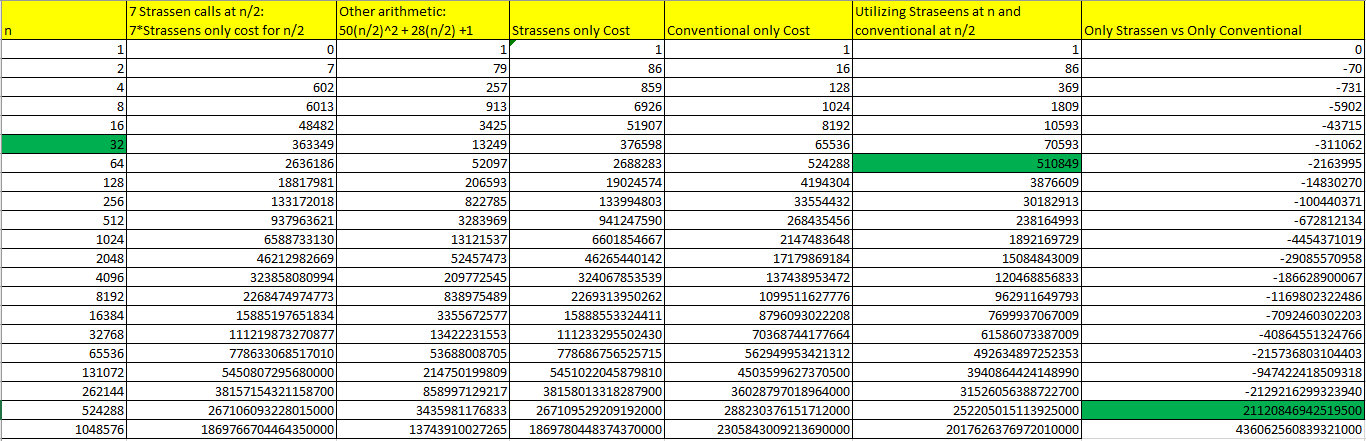
\includegraphics[width = 5in]{cost.png}
\newpage
What we can see here is that purely using Strassens over conventional doesn't become cost effective until a very large n value, ~524288. However, utilizing a crossover point, where we call Strassens at n and use conventional at n/2, we can see this becomes cost effective much sooner. At n=64, if we call Strassens, Strassens will make 7 calls to Conventional with input n/2 and also incur the cost of ~52097 for other arithmetic operations. However this proves to be lower then the cost of simply calling conventional with input n. As a result, this analysis would indicate that the crossover point is n=32. As at n=64, we would want to start off using Strassens. 

\subsection{Time trials} 
I also wanted to test things out myself and see if the above analysis made sense when doing time trials (average taken over 3 trials per cell). After running time trials with different crossover points, I got the below results. These results indicate that having a crossover point at n=64 is actually slightly better then n=32. I believe the reason for this is that the above analysis only took into account arithmetic operations. However, there were other operations that we did such as creating and setting variables which take time. The analysis above indicates that n=32 is the crossover point but when we look at the chart, we can see it's pretty close where using Strassens at n=64 and switch to conventional at n=32 only slightly beats out using just conventional. Given that, and the time analysis, I ultimately believe that the best crossover point is n=64 but it's very close and could just be machine dependent. \break

            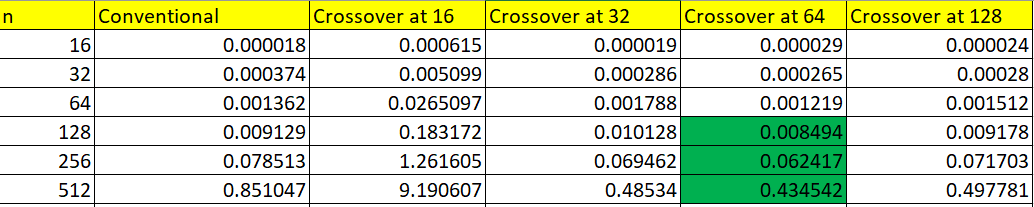
\includegraphics[width = 5in]{time.png} 
            
\subsection{Auto-grader unknown issue} 
I was experiencing an unknown issue with the autograder. When I set my crossover point at n=2, my code works and the auto-grader reports back correct results. It does report back that my code is running too slow for larger n values. This is understandable because the crossover point should be higher, (32 or 64). However, when I try to use a higher crossover point such as 32 or 64, the auto grader reports back that I have achieved the wrong results for dimensions 4x4, 5x5, 6x6, etc. This is rather odd because I've done multiple tests with different input files and from what I see they are reporting back the correct values and outputting the same output as when I have a crossover point of n=2. I tried this with negative values as well and still am getting the same results regardless of crossover point. 
In order to address this, I have two functions. One uses a pure version of Strassens that doesn't crossover at n=32. This is what will be used when the original input dimensions are 32 or lower. Anytime the input dimensions are higher, I utilize Strassens crossover which switches to conventional at n=32. This seems to work with the grading server however it is really odd as I could not find any bugs and the Strassens crossover function should be working on all inputs, as it seems to when I run locally.
            
\newpage

\section{Building code/optimizations/observations}
\subsection{Passing matrices}
One observation I quickly learned is that C++ does not allow you to create functions that accept matrices as input if I need the function to accept matrices of different sizes. I would have to declare the number of columns or rows to allow for this. To account for this, I started using pointers. Each pointer would point to a list of size n and each of the n elements of the list would be an n sized list. This would achieve the same results as a matrice and I could point to each list with a pointer. This is also good because it uses less space. By passing a pointer to a matrice, I do not need to pass the entire matrice to be stored in memory. This would take up much more space as we got to large n values. 
\subsection{Padding for odd sized matrices}
My method for dealing with odd sized matrices is to pad them with an additional column/row of 0's. During my very first implementation, I tried padding so that the original input matrices would be increased to a size of the next power of 2. For example, an input matrice of size 13 would be increased to size 16 which is a power of two. I realized that although this would work, it could nearly double the run time. For example, an input of n=257 would mean a padding of 255 rows/columns! This would take a lot longer to do. As a result, I switched to adding a row/column only when n was odd. As a result, I would add far fewer unnecessary rows/columns. As a result, I removed the below function as it was no longer needed which would find the next highest power of 2. 

            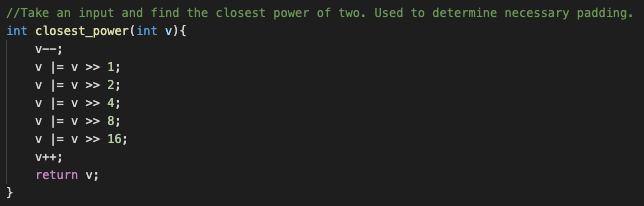
\includegraphics[width = 5in]{power.png} 
\newpage
\subsection{Counting arithmetic operations}
The instructions recommended that we count each arithmetic operation in order to determine the cost of running strassens given n. One thing I realized is how many times I was doing arithmetic operations again that could instead be saved as variables. The ultimate cost savings here would be small but could become more substantial for larger n. Here is an example where I utilized creating variables instead of redoing operations. If the analysis hadn't called for counting arithmetic operations, I likely would have repeated them. Here's an example. Previously the calculations for m and n were being redone multiple times every time we looped.  \break
            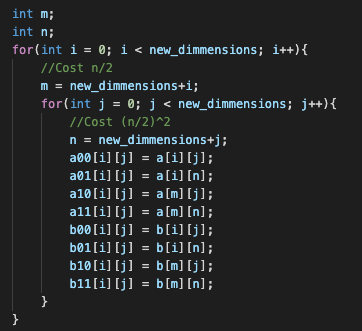
\includegraphics[width = 3in]{example.png} 
\newpage
\section{Representing Graphs}
In order to do this I created two functions called random and triangles. Random utilized the same random number generator I used from the first programming assignment to decide between 1 and 0. Triangles would create a new 1024x1024 matrice and then assign a value 1 or 0 based on the probability for each cell. I made sure to account for if an edge was already listed from i to j that it would also be marked the same for j to i. One mistake I made at first was assuming that the cell for a vertice to itself should be marked as 1. When I first did this, I was getting very large values that weren't close to the expected values. After I changed this so that each cell (x,x) was marked as 0, the number of triangles was in line with the expected values. I ran three trials for each and have the values listed below along with averages, rounding to the nearest integer . \break  \break
            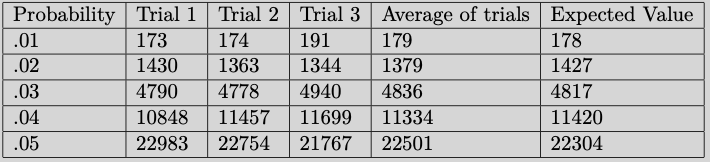
\includegraphics[width = 5in]{graphs.png} 


\endflushleft



\end{document} 